\ifdefined\ishandout
\documentclass[handout, 10pt]{beamer}
\else
\documentclass[10pt]{beamer}
\fi

%\usepackage[frenchb]{babel}
\usepackage[T1]{fontenc}
%\usepackage[utf8]{inputenc}
\usepackage{hyperref}
\usepackage{multirow}
\usepackage{listings}
\usepackage{fancyvrb}
\usepackage{tikz}
\usepackage{framed}
\usepackage{xmpmulti}
\usepackage{algorithm}
\usepackage{algorithmicx}
\usepackage{algpseudocode}
\usepackage{xcolor}
\usepackage{booktabs}
\usepackage{color, colortbl}
\ifdefined\ishandout
\usepackage{handoutWithNotes}
\fi
\usepackage{slashbox}
\usepackage{amsmath}
\usepackage{bm}
\usepackage{hhline}
\usepackage{pgfplots}
\usepackage{caption}
%\graphicspath{{../old/course-utrecht/fig/}{../old/course-utrecht/fig/L1/}{../old/course-utrecht/fig/L2/}{../old/course-utrecht/fig/L3/}} %Setting the graphicspath

\def\UrlBreaks{\do\/\do-}

\usetikzlibrary{shapes.geometric}
\usetikzlibrary{positioning}
\usetikzlibrary{shapes.arrows, chains}
\usetikzlibrary{arrows,calc}
\usetikzlibrary{shapes.multipart}
\usetikzlibrary{matrix}

\usepackage{array}
%\usetheme{Boadilla}
\usetheme[progressbar=frametitle]{metropolis}

\usefonttheme[onlymath]{serif}

\newcommand{\R}{\mathbb{R}}
%\newcommand{\C}{\mathbb{C}}
\newcommand{\N}{\mathbb{N}}
\newcommand{\Z}{\mathbb{Z}}
\newcommand{\E}{\mathbb{E}}
\newcommand{\Var}{\text{Var}}
\newcommand{\Cov}{\text{Cov}}
\ifdefined\ishandout
\pgfpagesuselayout{3 on 1 with notes}[a4paper,border shrink=5mm]
\usecolortheme{dove}
\else
%\usecolortheme{dolphin}
%\usecolortheme{crane}
\fi

\metroset{block=fill}

\lstnewenvironment{codeC}
{ \lstset{language=C,
    otherkeywords={printf,scanf}}
}
{}

\ifdefined\ishandout
\definecolor{mygreen}{rgb}{0,0,0}
\definecolor{mymauve}{rgb}{0,0,0}
\definecolor{myblue}{rgb}{0,0,0}
\else
\definecolor{mygreen}{rgb}{0,0.6,0}
\definecolor{mymauve}{rgb}{0.58,0,0.82}
\definecolor{myblue}{rgb}{0,0,1}

\fi

%% Notes
%\setbeameroption{show only notes}


\definecolor{mygray}{rgb}{0.5,0.5,0.5}

\lstset{ language=Python,%
  backgroundcolor=\color{white},   % choose the background color; you must add \usepackage{color} or \usepackage{xcolor}
  basicstyle=\footnotesize,        % the size of the fonts that are used for the code
  breakatwhitespace=false,         % sets if automatic breaks should only happen at whitespace
  breaklines=true,                 % sets automatic line breaking
  captionpos=b,                    % sets the caption-position to bottom
  commentstyle=\color{mygreen},    % comment style
  deletekeywords={...},            % if you want to delete keywords from the given language
  escapeinside={\%*}{*)},          % if you want to add LaTeX within your code
  extendedchars=true,              % lets you use non-ASCII characters; for 8-bits encodings only, does not work with UTF-8
  frame=tb,	                   % adds a frame around the code
  keepspaces=true,                 % keeps spaces in text, useful for keeping indentation of code (possibly needs columns=flexible)
  keywordstyle=\color{blue},       % keyword style
  otherkeywords={*,...},           % if you want to add more keywords to the set
  numbers=none,                    % where to put the line-numbers; possible values are (none, left, right)
  numbersep=5pt,                   % how far the line-numbers are from the code
  numberstyle=\tiny\color{mygray}, % the style that is used for the line-numbers
  rulecolor=\color{black},         % if not set, the frame-color may be changed on line-breaks within not-black text (e.g. comments (green here))
  showspaces=false,                % show spaces everywhere adding particular underscores; it overrides 'showstringspaces'
  showstringspaces=false,          % underline spaces within strings only
  showtabs=false,                  % show tabs within strings adding particular underscores
  stepnumber=2,                    % the step between two line-numbers. If it's 1, each line will be numbered
  stringstyle=\color{mymauve},     % string literal style
  tabsize=3,	                   % sets default tabsize to 2 spaces
  title=\lstname                   % show the filename of files included with \lstinputlisting; also try caption instead of title
}
%\lstset{language=Python,
% breakatwhitespace=false,         % sets if automatic breaks should only happen at whitespace
%  breaklines=true,                 % sets automatic line breaking
%  captionpos=b,                
%%commentstyle=\itshape\color{mymauve},
%%keywordstyle=\bfseries\color{myblue},
%numbers=left,                    % where to put the line-numbers; possible values are (none, left, right)
%  numbersep=8pt,                   % how far the line-numbers are from the code
%  numberstyle=\tiny\color{mygray}, % the style that is used for the line-numbers
%%  rulecolor=\color{black},         % if not set, the frame-color may be changed on line-breaks within not-black text (e.g. comments (green here))
%  showspaces=false,                % show spaces everywhere adding particular underscores; it overrides 'showstringspaces'
%%  showstringspaces=false,          % underline spaces within strings only
%  showtabs=false,                  % show tabs within strings adding particular underscores
%  stepnumber=2,                    % the step between two line-numbers. If it's 1, each line will be numbered
%%  stringstyle=\color{mygreen},     % string literal style
%  tabsize=2 
%}
\ifdefined\ishandout
\newcommand{\red}{\textbf}
\else
\newcommand{\red}{\textcolor{red}}
\fi
%\newcommand \emph
%Default size : 12.8 cm * 9.6 cm

\newcommand{\tmark}[1]{\tikz[remember picture, baseline=-.5ex]{\coordinate(#1);}}

\definecolor{bluegreen}{RGB}{0,149,182}


%\newcommand{\output}[1]{
\setbeamertemplate{navigation symbols}{}
\newcommand{\bvrb}{\Verb[commandchars=£µ§,formatcom=\color{bluegreen}]}
\newcommand{\footvrb}{\footnotesize\Verb}
\newcommand{\vrbalert}[2][]{\visible<#1>{#2}}
%%% Commande pour les listes/arbres
\newcommand{\mvide}{\nodepart{one} \nodepart{two}}
\newcommand{\tvide}{\nodepart{one} \nodepart{two} \nodepart{three}}
\newcommand{\rref}[1][]{\hfill{\scriptsize\textit{#1}}}

%%Fin des commandes pour les listes/arbres.



%%% Paramètres du cours (à régler)
%Numéro du cours
\newcommand{\nb}{1}

\title[Machine Learning]{Machine learning and physical (Earth system) modelling - course 4}
\author[J. Brajard]{julien.brajard@nersc.no}
\institute[NERSC]{NERSC\\
slides+notebook: \url{https://github.com/nansencenter/nersc_ml_course}}
\date{October 2021}

\begin{document}
%%%%%%%%%%%%%%%%%%%%% SLIDES DE TITRE
\begin{frame}
\titlepage
\end{frame}

\begin{frame}[allowframebreaks]{Table of contents}
  \setbeamertemplate{section in toc}[sections numbered]
  \tableofcontents[hideallsubsections]
\end{frame}


%%%%%%%%%%%%%%%%%%%%%%%%%%%%%%%%%%%%%%%%%%
\section{Neural Networks}

\begin{frame}
  \frametitle{The perceptron : an artificial neuron}
  \begin{tikzpicture}[
    basic/.style={draw,fill=blue!20,text width=1em,text badly centered},
    input/.style={basic,circle},
    weights/.style={basic,rectangle},
functions/.style={basic,circle,fill=blue!10},
]
        \node[functions] (center) {};
        \node[below of=center,font=\scriptsize,text width=4em] {Activation function};
        \draw[thick] (0.5em,0.5em) -- (0,0.5em) -- (0,-0.5em) -- (-0.5em,-0.5em);
      %  \draw (0em,0.75em) -- (0em,-0.75em);
      %  \draw (0.75em,0em) -- (-0.75em,0em);
        \node[right of=center, anchor = west] (right) {$y=$ 0 ou 1};
            \path[draw,->] (center) -- (right);
        \node[functions,left=3em of center] (left) {$\sum$};
            \path[draw,->] (left) -- (center);
%        \node[weights,left=3em of left] (2) {$w_2$} -- (2) 
            \node[input,left= 4em of left] (l2) {$x_2$};
%            \path[draw,->] (l2) -- (2);
            \path[draw,->] (l2) -- node[above,midway]{$w_2$}(left);
        \node[below of=l2] (dots) {$\vdots$} ;
%(dots) node[left of=dots] (ldots) {$\vdots$};
%        \node[weights,below of=dots] (n) {$w_n$} -- (n) 
\node[input,below of=dots] (ln) {$x_n$};
%            \path[draw,->] (ln) -- (n);
            \path[draw,->] (ln) -- node[above,midway]{$w_n$}(left);
%        \node[weights,above of=2] (1) {$w_1$} -- (1) 
            \node[input,above of=l2] (l1) {$x_1$};
%            \path[draw,->] (l1) -- (1);
            \path[draw,->] (l1) -- node[above,midway]{$w_1$}(left);
%        \node[weights,above of=1] (0) {$w_0$} -- (0) 
\node[input,above of=l1] (l0) {$1$};
%            \path[draw,->] (l0) -- (0);
            \path[draw,->] (l0) -- node[above,midway]{$w_0$}(left);
        \node[below of=ln,font=\scriptsize](lin) {inputs};
        \node[right of=lin,xshift=+1em,font=\scriptsize] {weights};
    \end{tikzpicture}
\begin{block}{Computation}
$
y = f\left( w_0 + w_1. x_1 + w_2. x_2 +  \dots + w_n. x_n \right) = f\left( w_0 + \sum_{i=1}^n w_i.x_i\right)
$
\end{block}
\end{frame}

\begin{frame}{Some remarks}
\begin{itemize}[<+->]
    \item Inputs $x_i$ are the different features of the data
    \item Weight $w_i$ are the parameters of the model to optimize
    \item If the activation function is identity, it is equivalent to a linear regression
\end{itemize}
\visible<4->{
\begin{block}{}
More complexe models are build by combining several perceptrons
\end{block}
}

\end{frame}


\begin{frame}{Multi-layer perceptron (Densely connected layers)}
    \def\layersep{1.5cm}

\begin{tikzpicture}[
   shorten >=1pt,->,
   draw=black!50,
    node distance=\layersep,
    every pin edge/.style={<-,shorten <=1pt},
    neuron/.style={circle,fill=black!25,minimum size=17pt,inner sep=0pt},
    input neuron/.style={neuron, fill=green!50},
    output neuron/.style={neuron, fill=red!50},
    hidden neuron/.style={neuron, fill=blue!50},
    annot/.style={text width=4em, text centered}
]

    % Draw the input layer nodes
    \foreach \name / \y in {1,...,4}
    % This is the same as writing \foreach \name / \y in {1/1,2/2,3/3,4/4}
        \node[input neuron, pin=left:Feature \#\y] (I-\name) at (0,-\y) {};

    % set number of hidden layers
    \newcommand\Nhidden{3}

    % Draw the hidden layer nodes
    \foreach \N in {1,...,\Nhidden} {
       \foreach \y in {1,...,5} {
          \path[yshift=0.5cm]
              node[hidden neuron] (H\N-\y) at (\N*\layersep,-\y cm) {};
           }
    \node[annot,above of=H\N-1, node distance=1cm] (hl\N) {Hidden layer \N};
    }

    % Draw the output layer node
    \node[output neuron,pin={[pin edge={->}]right:Output}, right of=H\Nhidden-3] (O) {};

    % Connect every node in the input layer with every node in the
    % hidden layer.
    \foreach \source in {1,...,4}
        \foreach \dest in {1,...,5}
            \path (I-\source) edge (H1-\dest);

    % connect all hidden stuff
    \foreach [remember=\N as \lastN (initially 1)] \N in {2,...,\Nhidden}
       \foreach \source in {1,...,5}
           \foreach \dest in {1,...,5}
               \path (H\lastN-\source) edge (H\N-\dest);

    % Connect every node in the hidden layer with the output layer
    \foreach \source in {1,...,5}
        \path (H\Nhidden-\source) edge (O);

    % Annotate the layers

    \node[annot,left of=hl1] {Input layer};
    \node[annot,right of=hl\Nhidden] {Output layer};
\end{tikzpicture}
\end{frame}

\begin{frame}{Most usual activation functions}
\begin{columns}
\column{.5\textwidth}
    \begin{figure}
        \centering
        Linear\\
        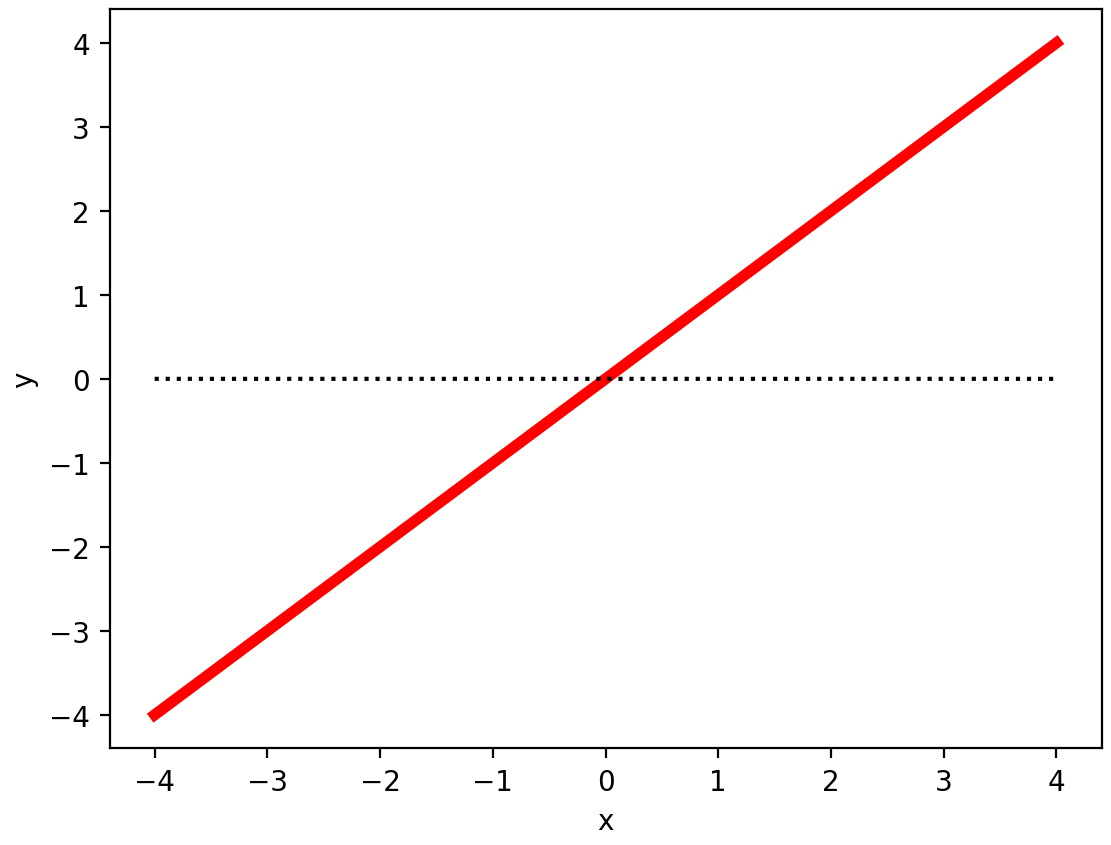
\includegraphics[width=.85\textwidth]{figs/activ-linear.png}\\
        ReLU\\
        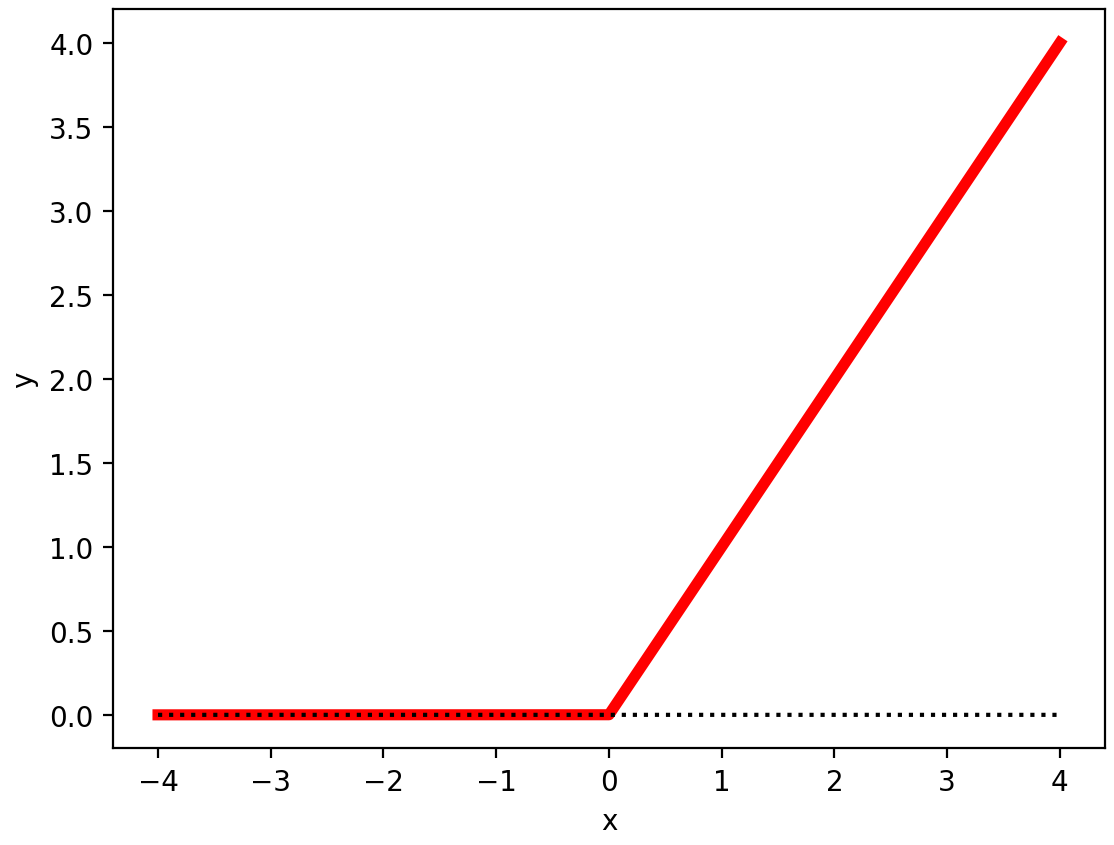
\includegraphics[width=.85\textwidth]{figs/activ-relu.png}\\

    \end{figure}
\column{.5\textwidth}
    \begin{figure}
     \centering
        Hyperbolic tangent\\
        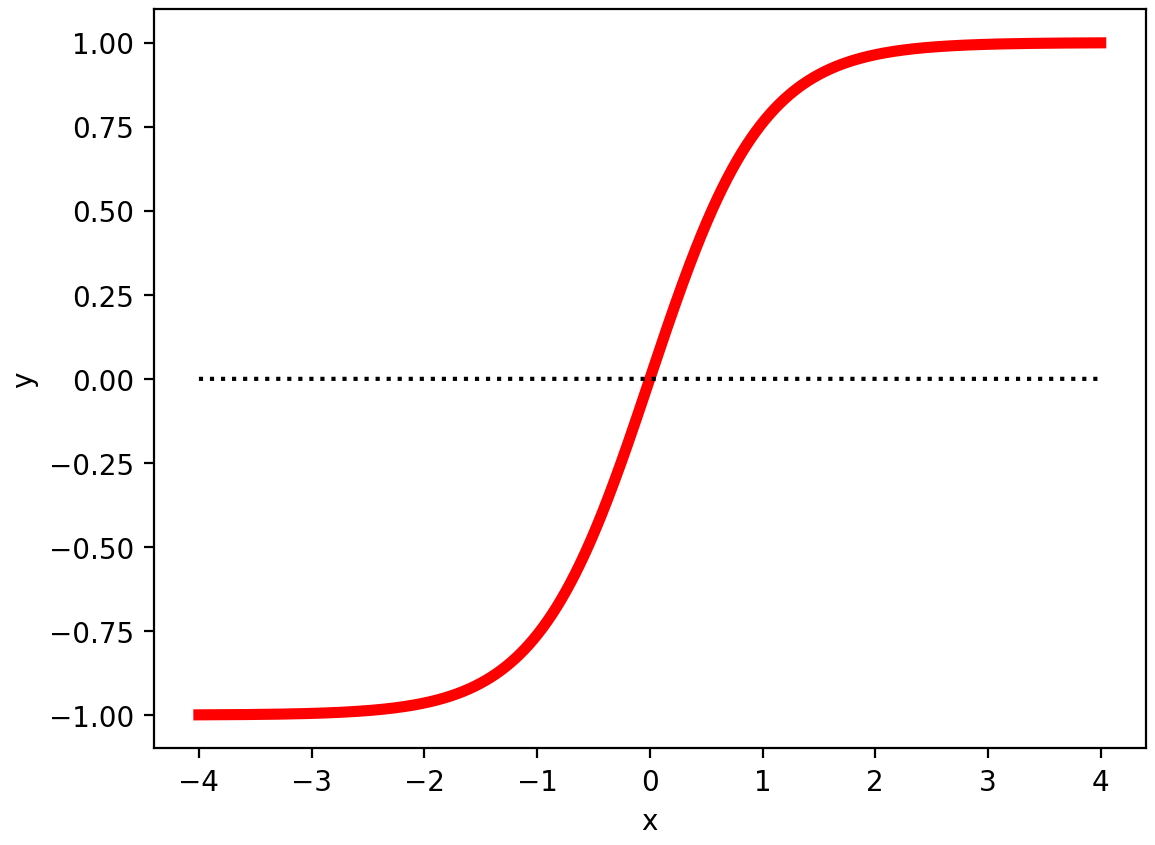
\includegraphics[width=.85\textwidth]{figs/activ-tanh.png}\\
       Sigmoid\\
        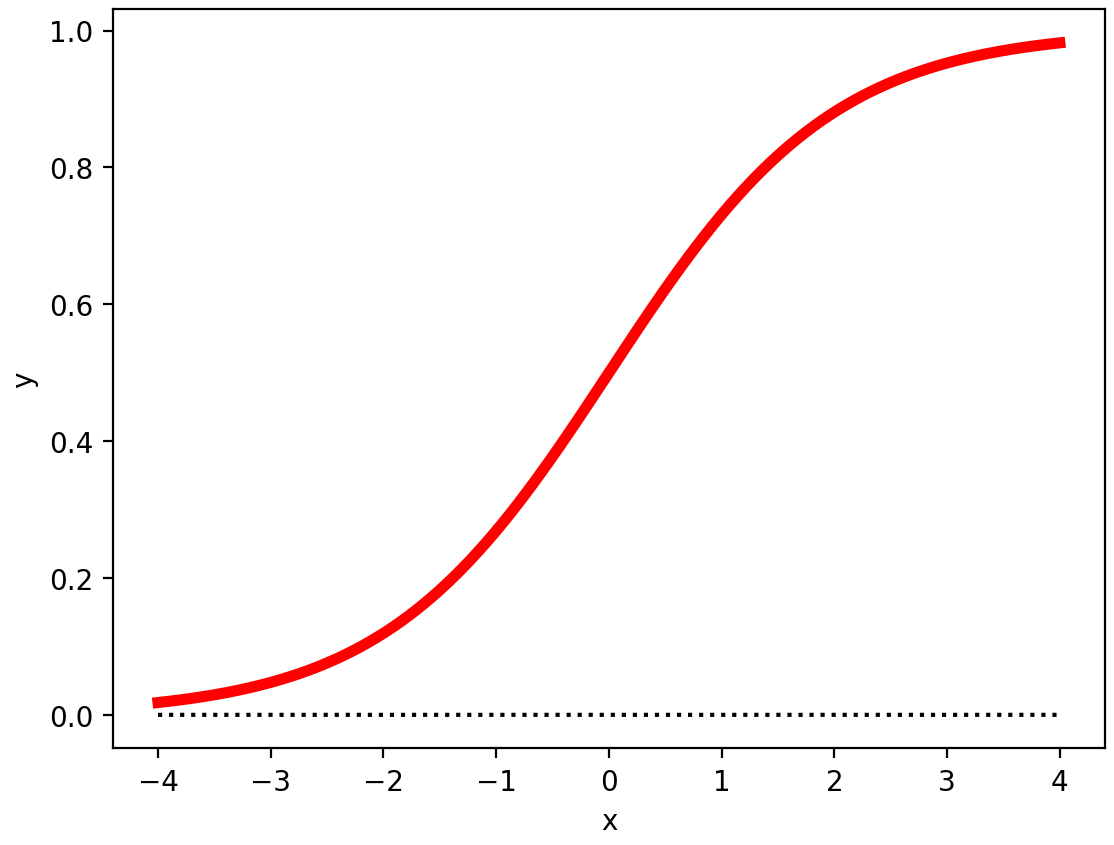
\includegraphics[width=.85\textwidth]{figs/activ-sigmoid.png}\\

    \end{figure}
\end{columns}
\end{frame}


\begin{frame}{New fancy activation functions}
\begin{columns}
\column{.5\textwidth}
    \begin{figure}
        \centering
        Leaky-ReLU\\
        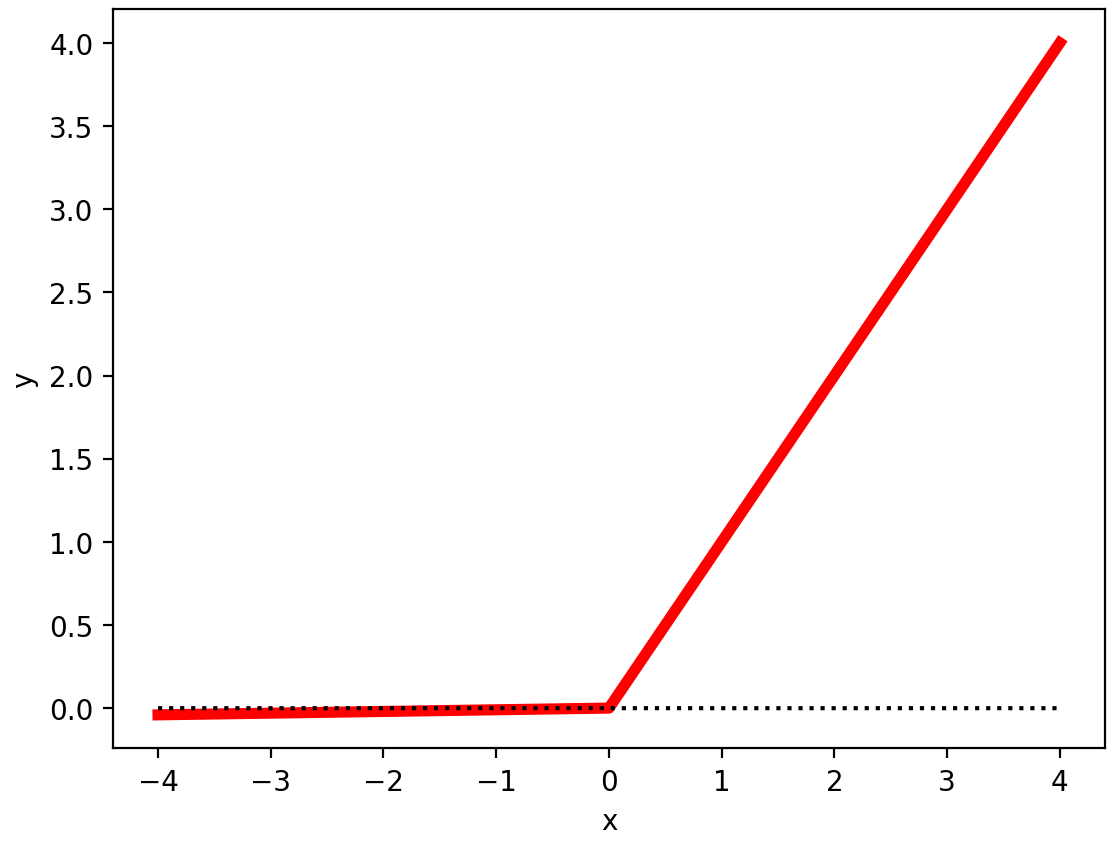
\includegraphics[width=.85\textwidth]{figs/activ-l-relu.png}\\
      

    \end{figure}
\column{.5\textwidth}
    \begin{figure}
     \centering
        Swish\\
        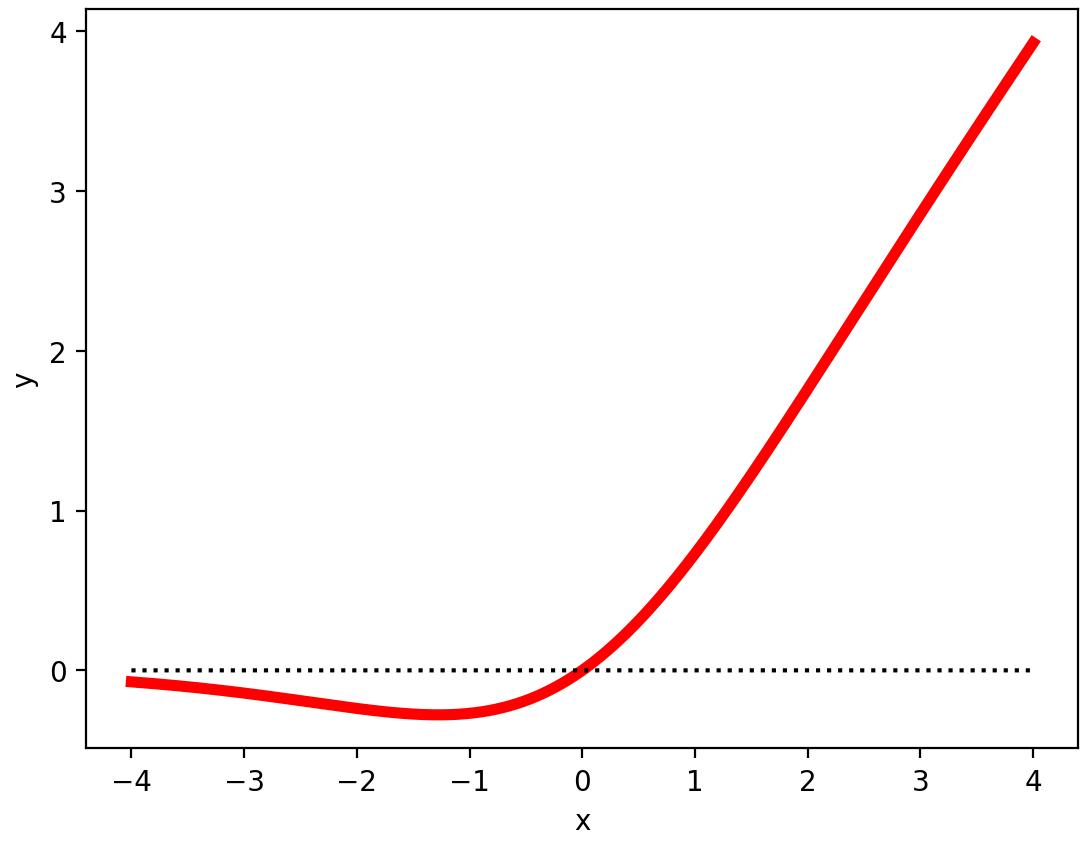
\includegraphics[width=.85\textwidth]{figs/activ-swish.png}\\
     

    \end{figure}
\end{columns}
\end{frame}


\begin{frame}{Classification and regression loss}
  
   \begin{columns}
   \column{.5\textwidth}
   \alert{Regression}
   \begin{itemize}
       \item Last layer:\\
       linear or hyperbolic tangent
       \item Loss function:\\
       $$L(\hat{y},y) = \sum_i (\hat{y}_i-y_i)^2$$
   \end{itemize}
   \pause
\column{.5\textwidth}
       \alert{Classification}
   \begin{itemize}
       \item Last layer:\\
       Soft-max
       $$
       p_j=f_j(\mathbf{h}) = \frac{e^{h_j}}{\sum_k e^{h_k}}
       $$
       
       \item Loss function:\\
       Negative crossentropy
       $$L(p,y) = -\sum_i \sum_j y_{i,j}.\log{p_{i,j}}$$
   \end{itemize}
   \end{columns}
\end{frame}

\begin{frame}{Classification loss (binary case)}
Objective: binary classification (the model determine if the input feature is in a class or not)\\
\vspace{1em}

Exemple: Try to know if an image is a cat or not.\\
\vspace{1em}

Dataset:

\begin{table}[]
    \centering
    \begin{tabular}{ccccc}
        {\bf x (feature)} &
         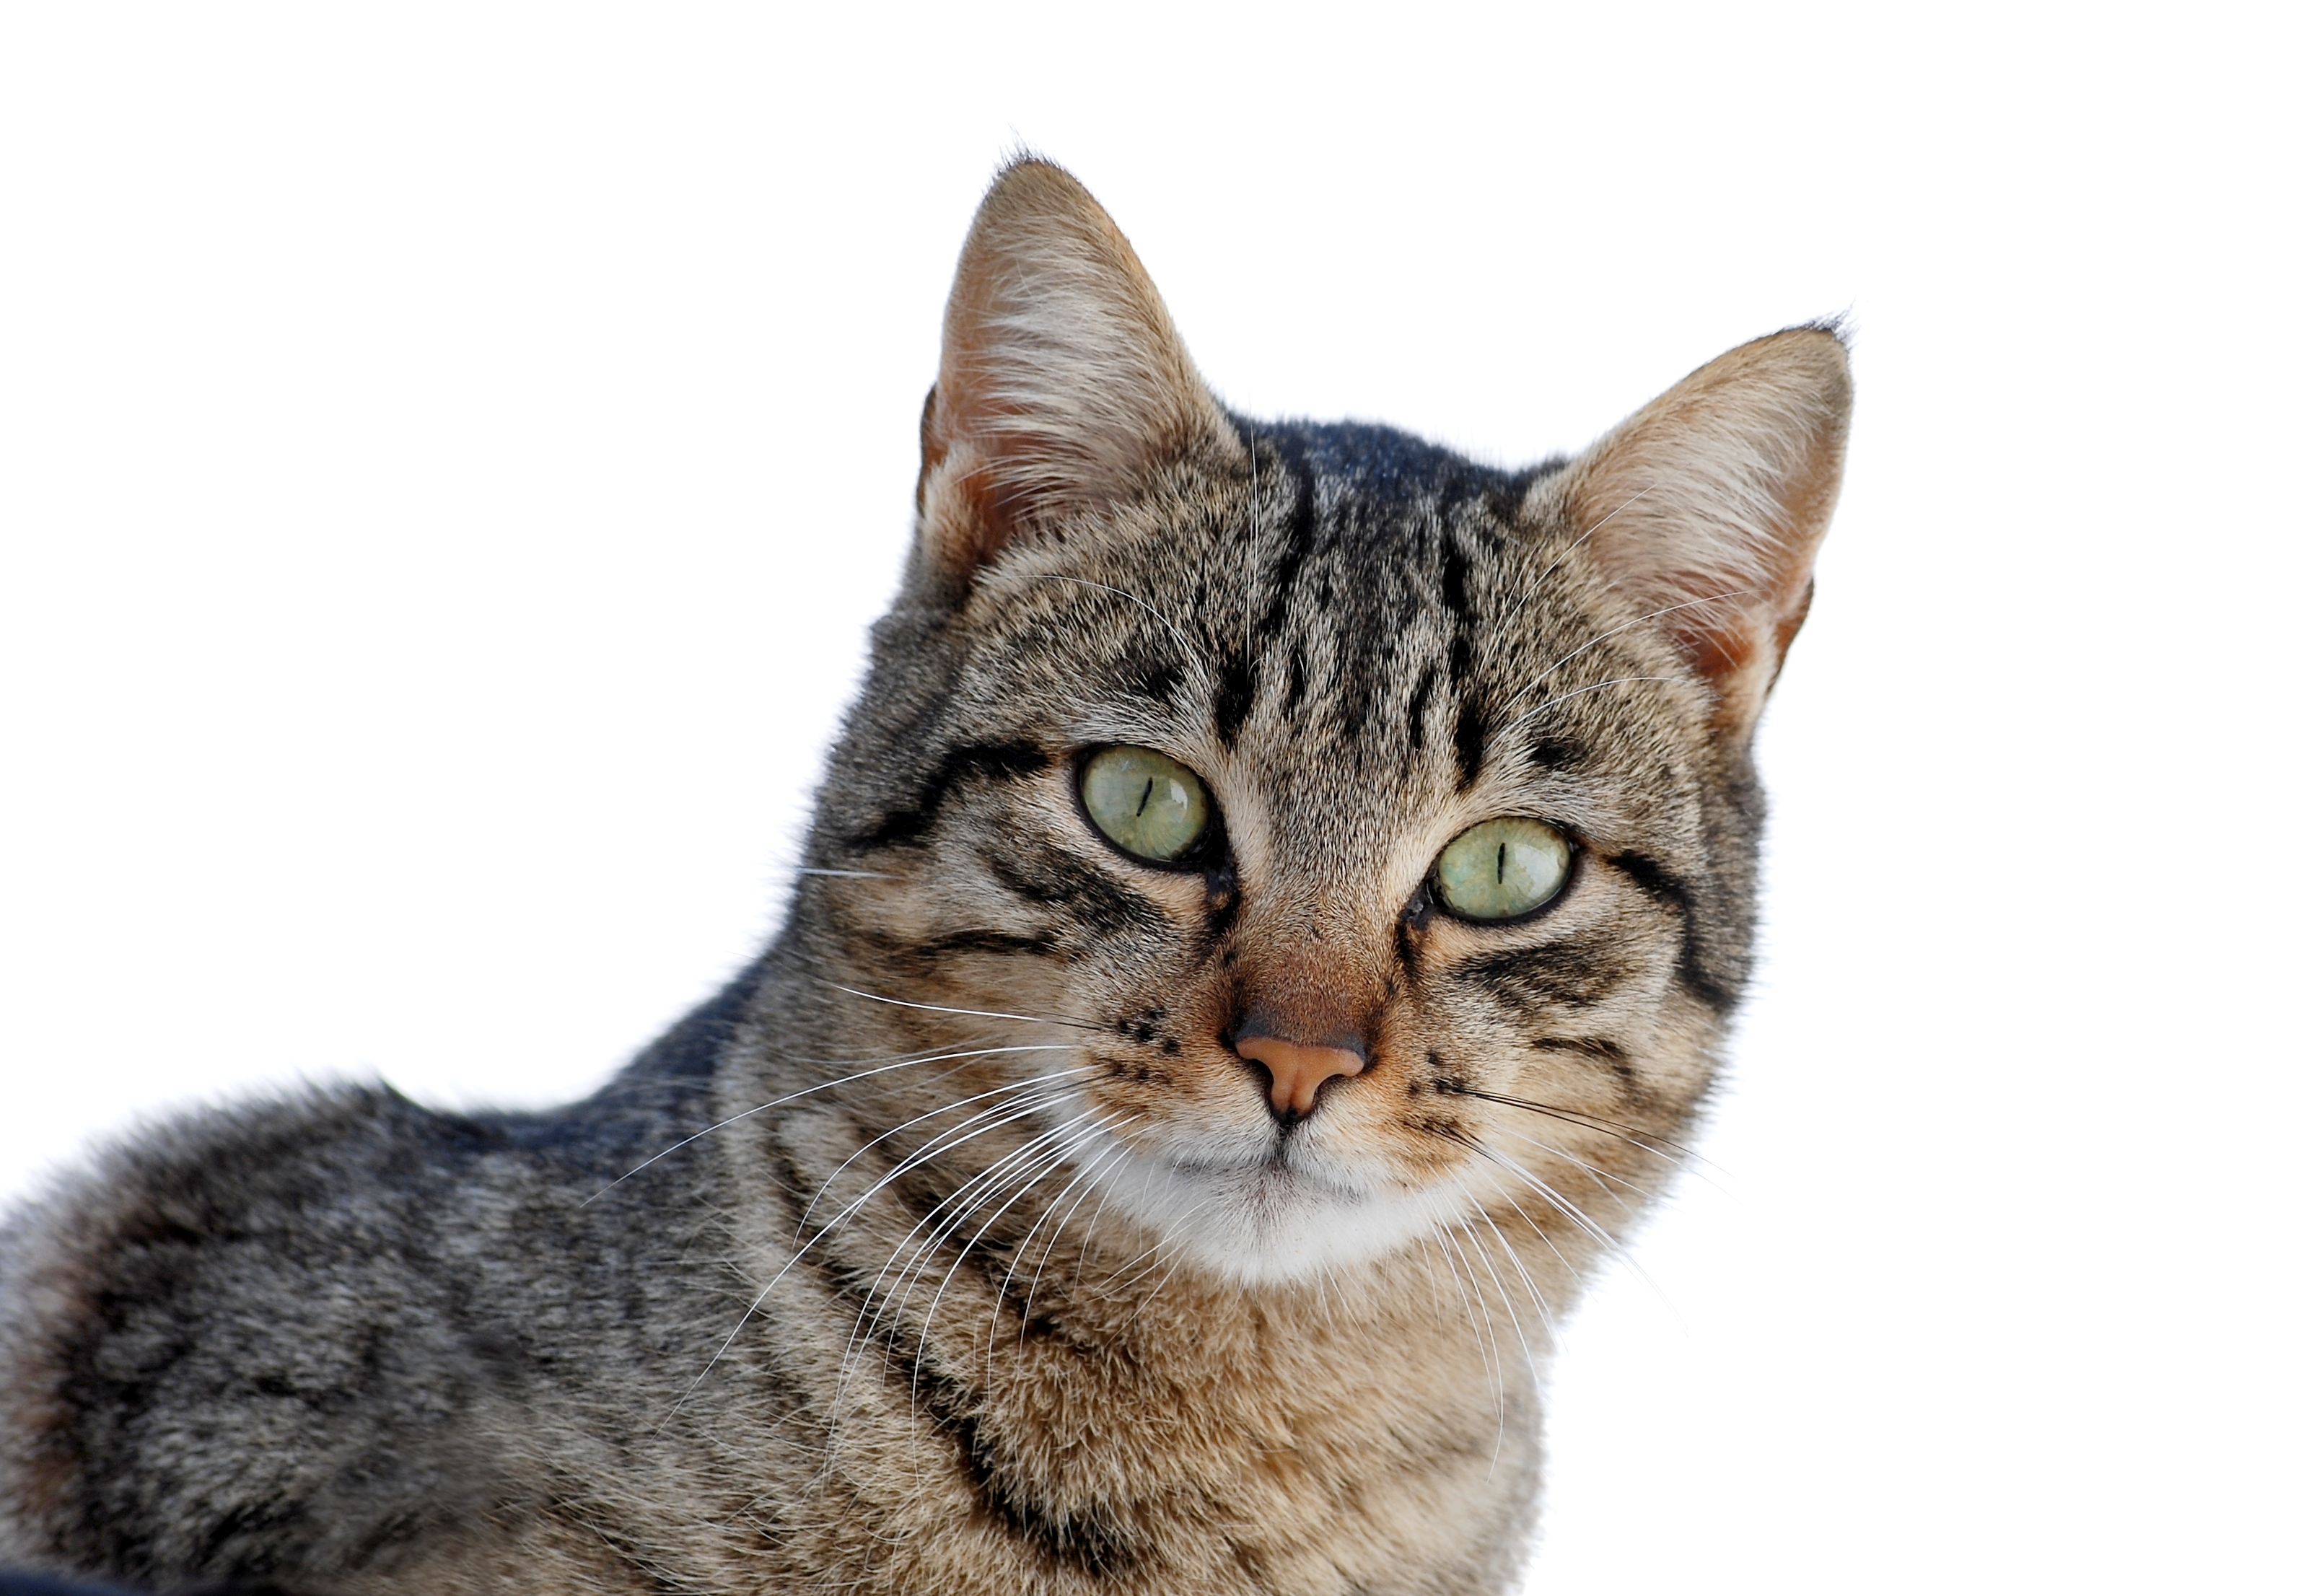
\includegraphics[width=.2\textwidth]{figs/cat1.jpg}& 
         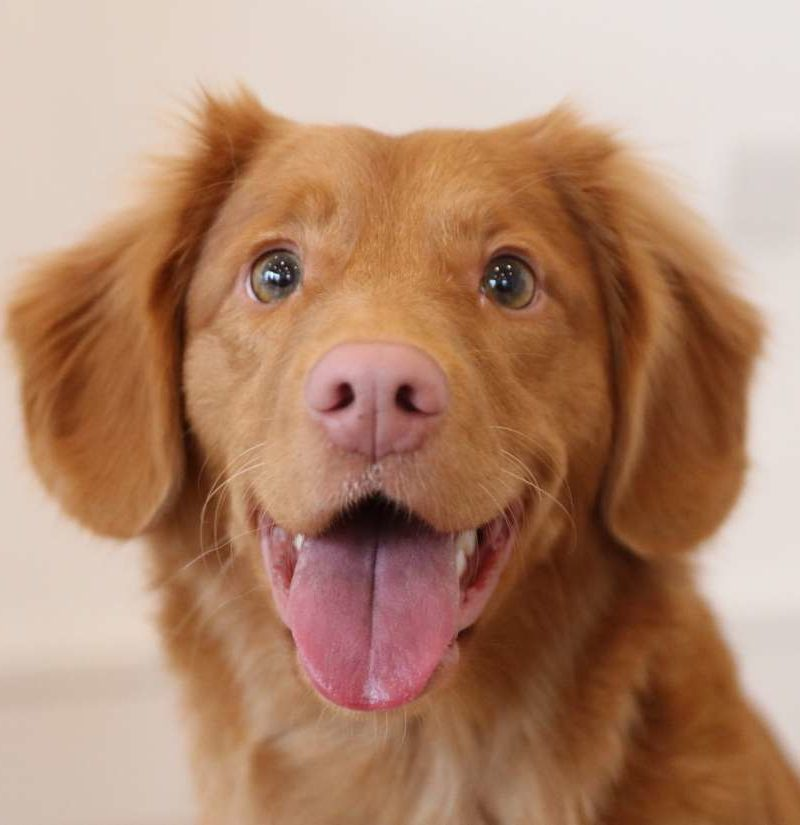
\includegraphics[width=.2\textwidth]{figs/dog1.jpg}&
         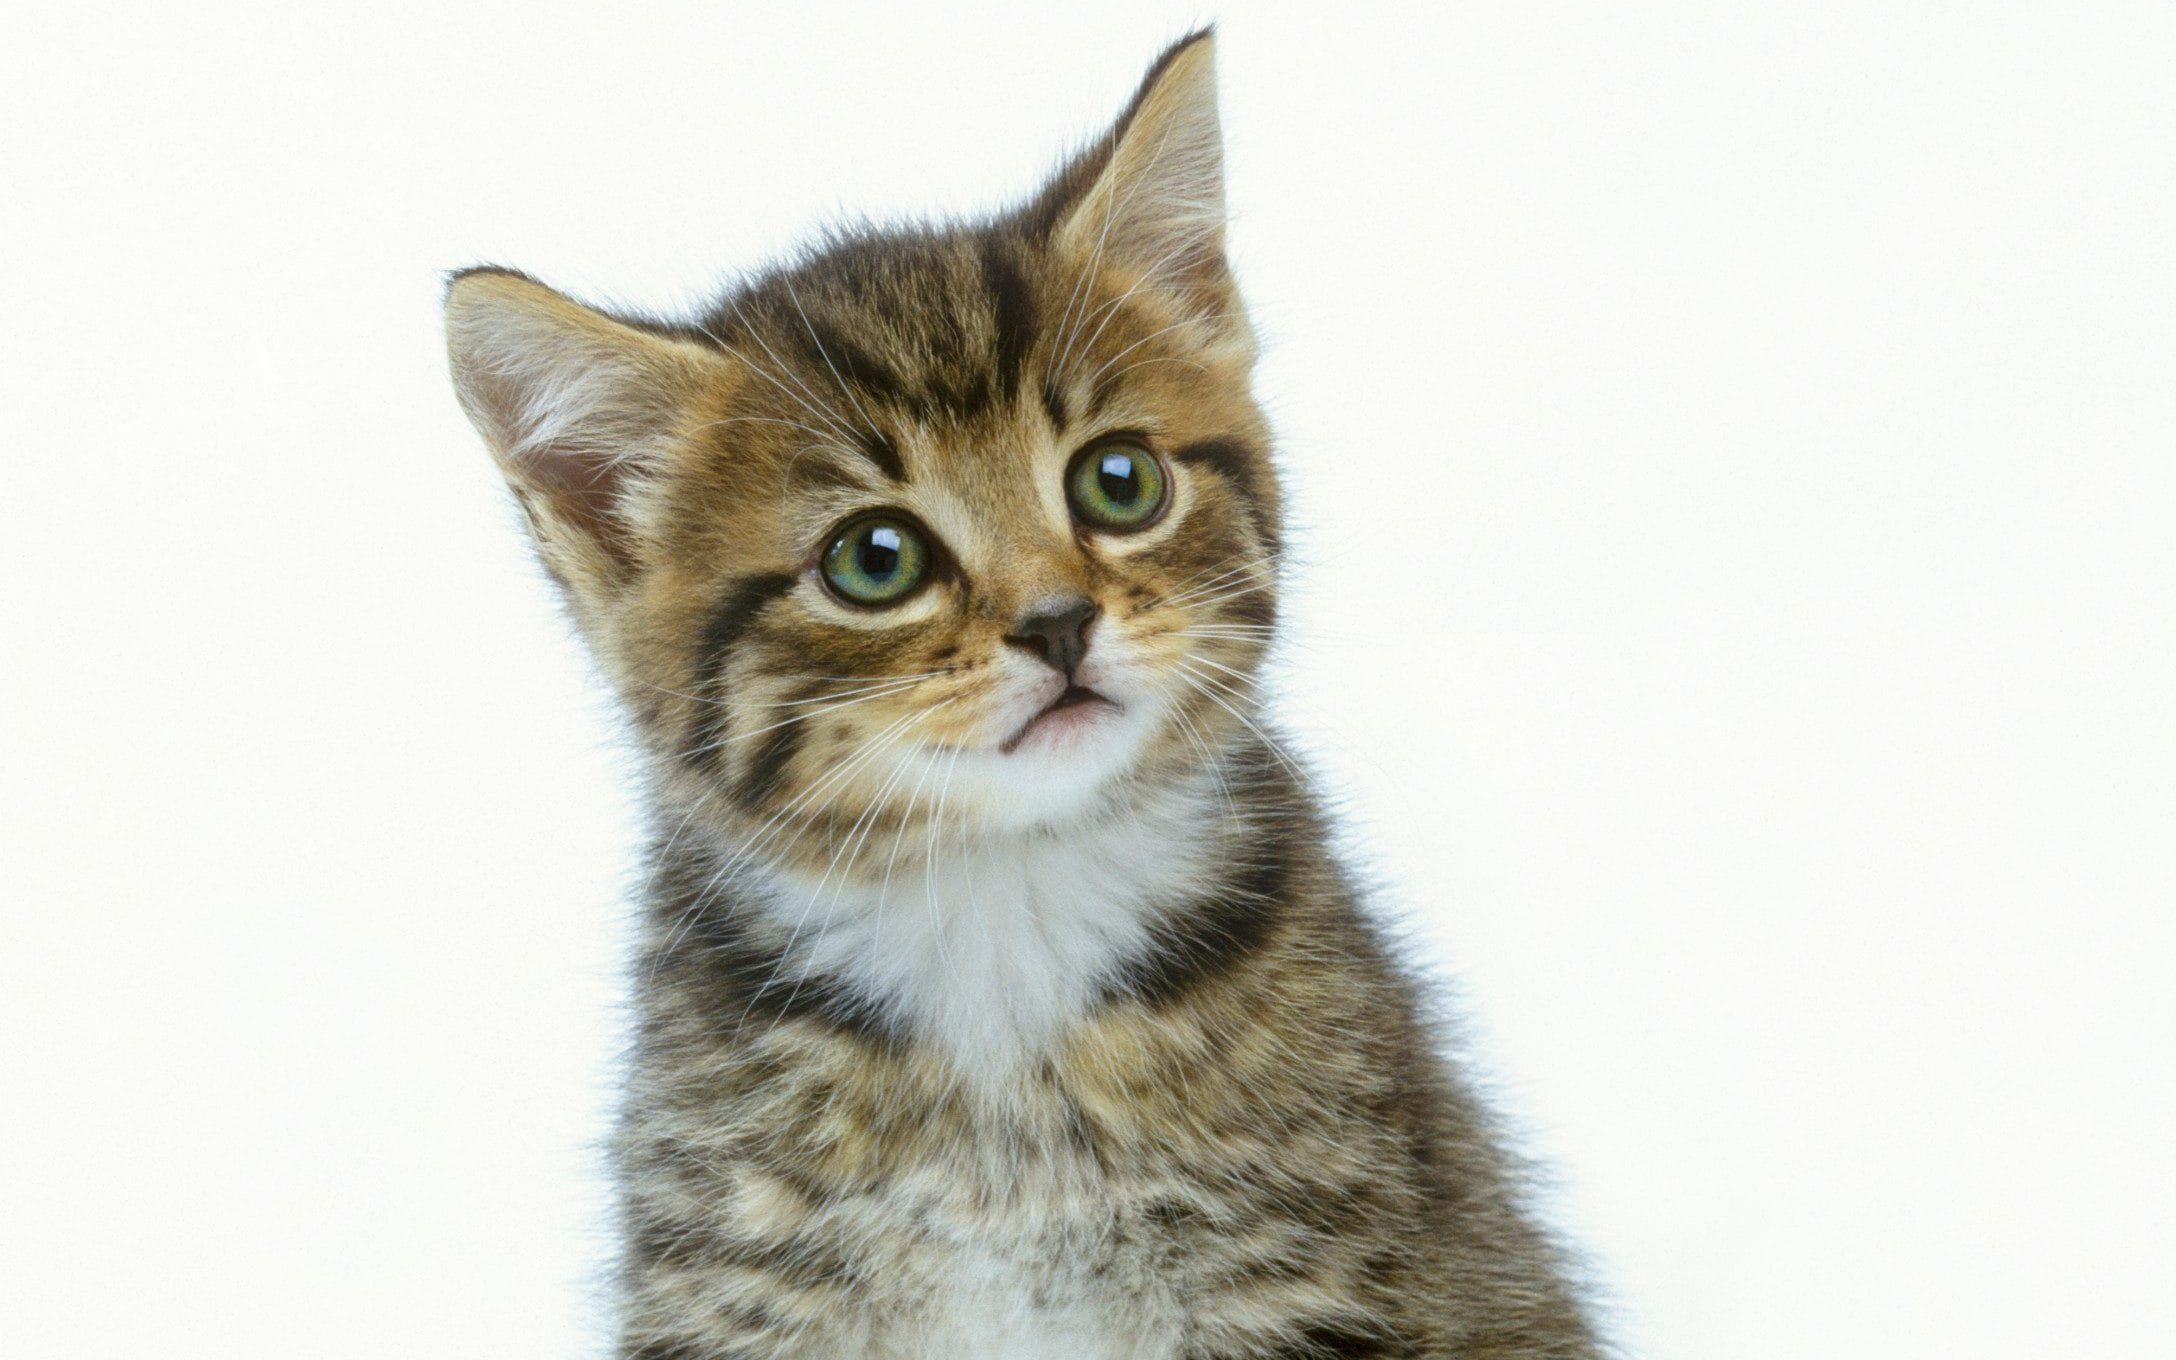
\includegraphics[width=.2\textwidth]{figs/cat2.jpg}&
         ...
         \\
        {\bf y (target)} & Cat & Dog & Cat & ...\\
    \end{tabular}
\end{table}

\end{frame}

\begin{frame}{How to proceed?}

\begin{enumerate}[<+->]
    \item Encode the targets (1 for cat, 0 otherwise)
    \begin{table}[]
    \centering
    \begin{tabular}{ccccc}
    
        {\bf y (target)} & Cat & Dog & Cat & ...\\
         {\bf y (encoded)} & 1 & 0 & 1 & ...\\
        
    \end{tabular}
\end{table}
    \item Design a model with \alert{\bf one output } and use the \alert{\bf sigmoid} as output activation function of your model $f(x)$, so $0 < f(x) < 1$.\\
    Rule: if $f(x)>\frac{1}{2}$, classify as ''Cat''.\\
    \alert{\bf f(x) is interpreted as the probability of the image x to be a cat.}
    \item Loss function to minimize is binary cross entropy:
    $$
    L = -\sum y_i \cdot \log(f(x_i)) + (1-y_i)\cdot \log (1-f(x_i))
    $$
\end{enumerate}    
\end{frame}

\begin{frame}{Classification loss (multiclass)}
Objective:  classification (the model determine in which class the input feature (more than 2 classes))\\
\vspace{1em}

Exemple: Try to know if an image is a cat, a dog or a duck.\\
\vspace{1em}

Dataset:

\begin{table}[]
    \centering
    \begin{tabular}{ccccc}
        {\bf x (feature)} &
         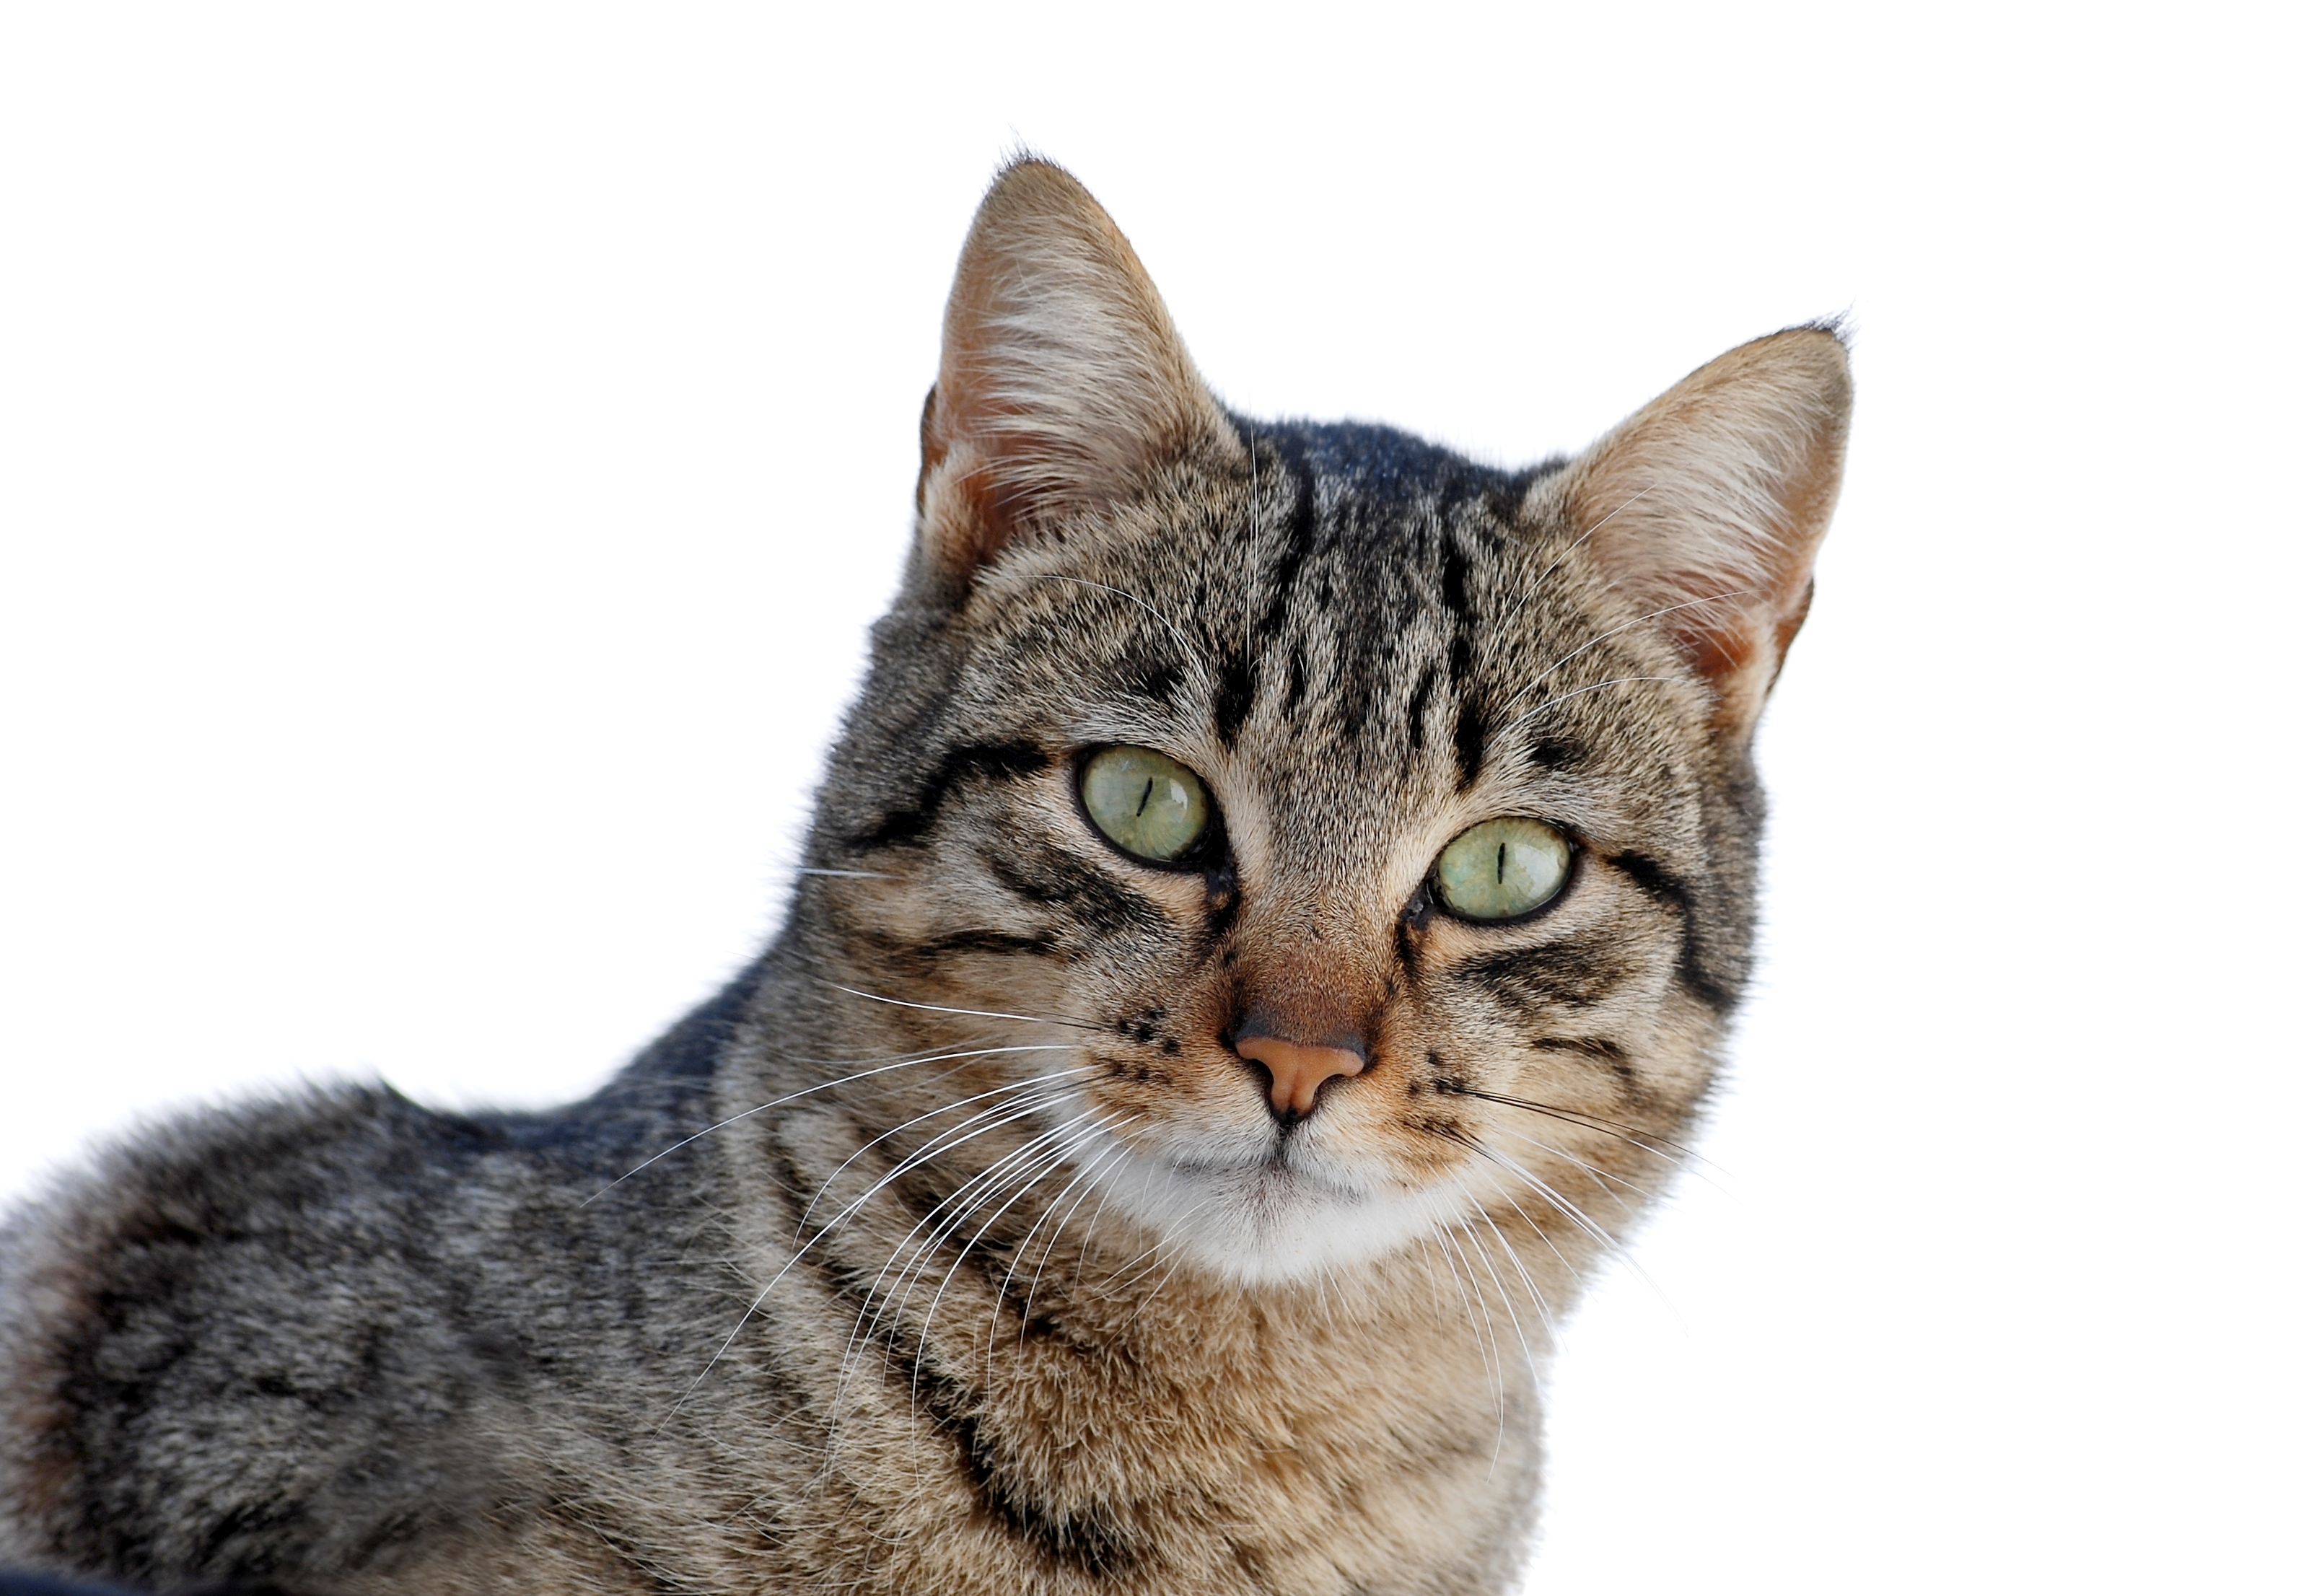
\includegraphics[width=.2\textwidth]{figs/cat1.jpg}& 
         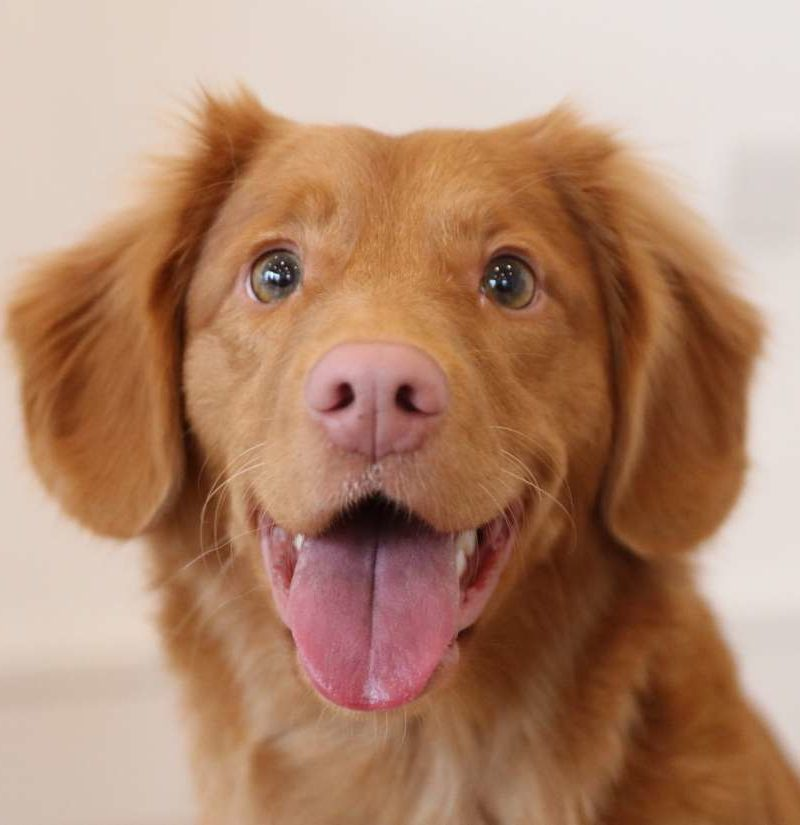
\includegraphics[width=.2\textwidth]{figs/dog1.jpg}&
         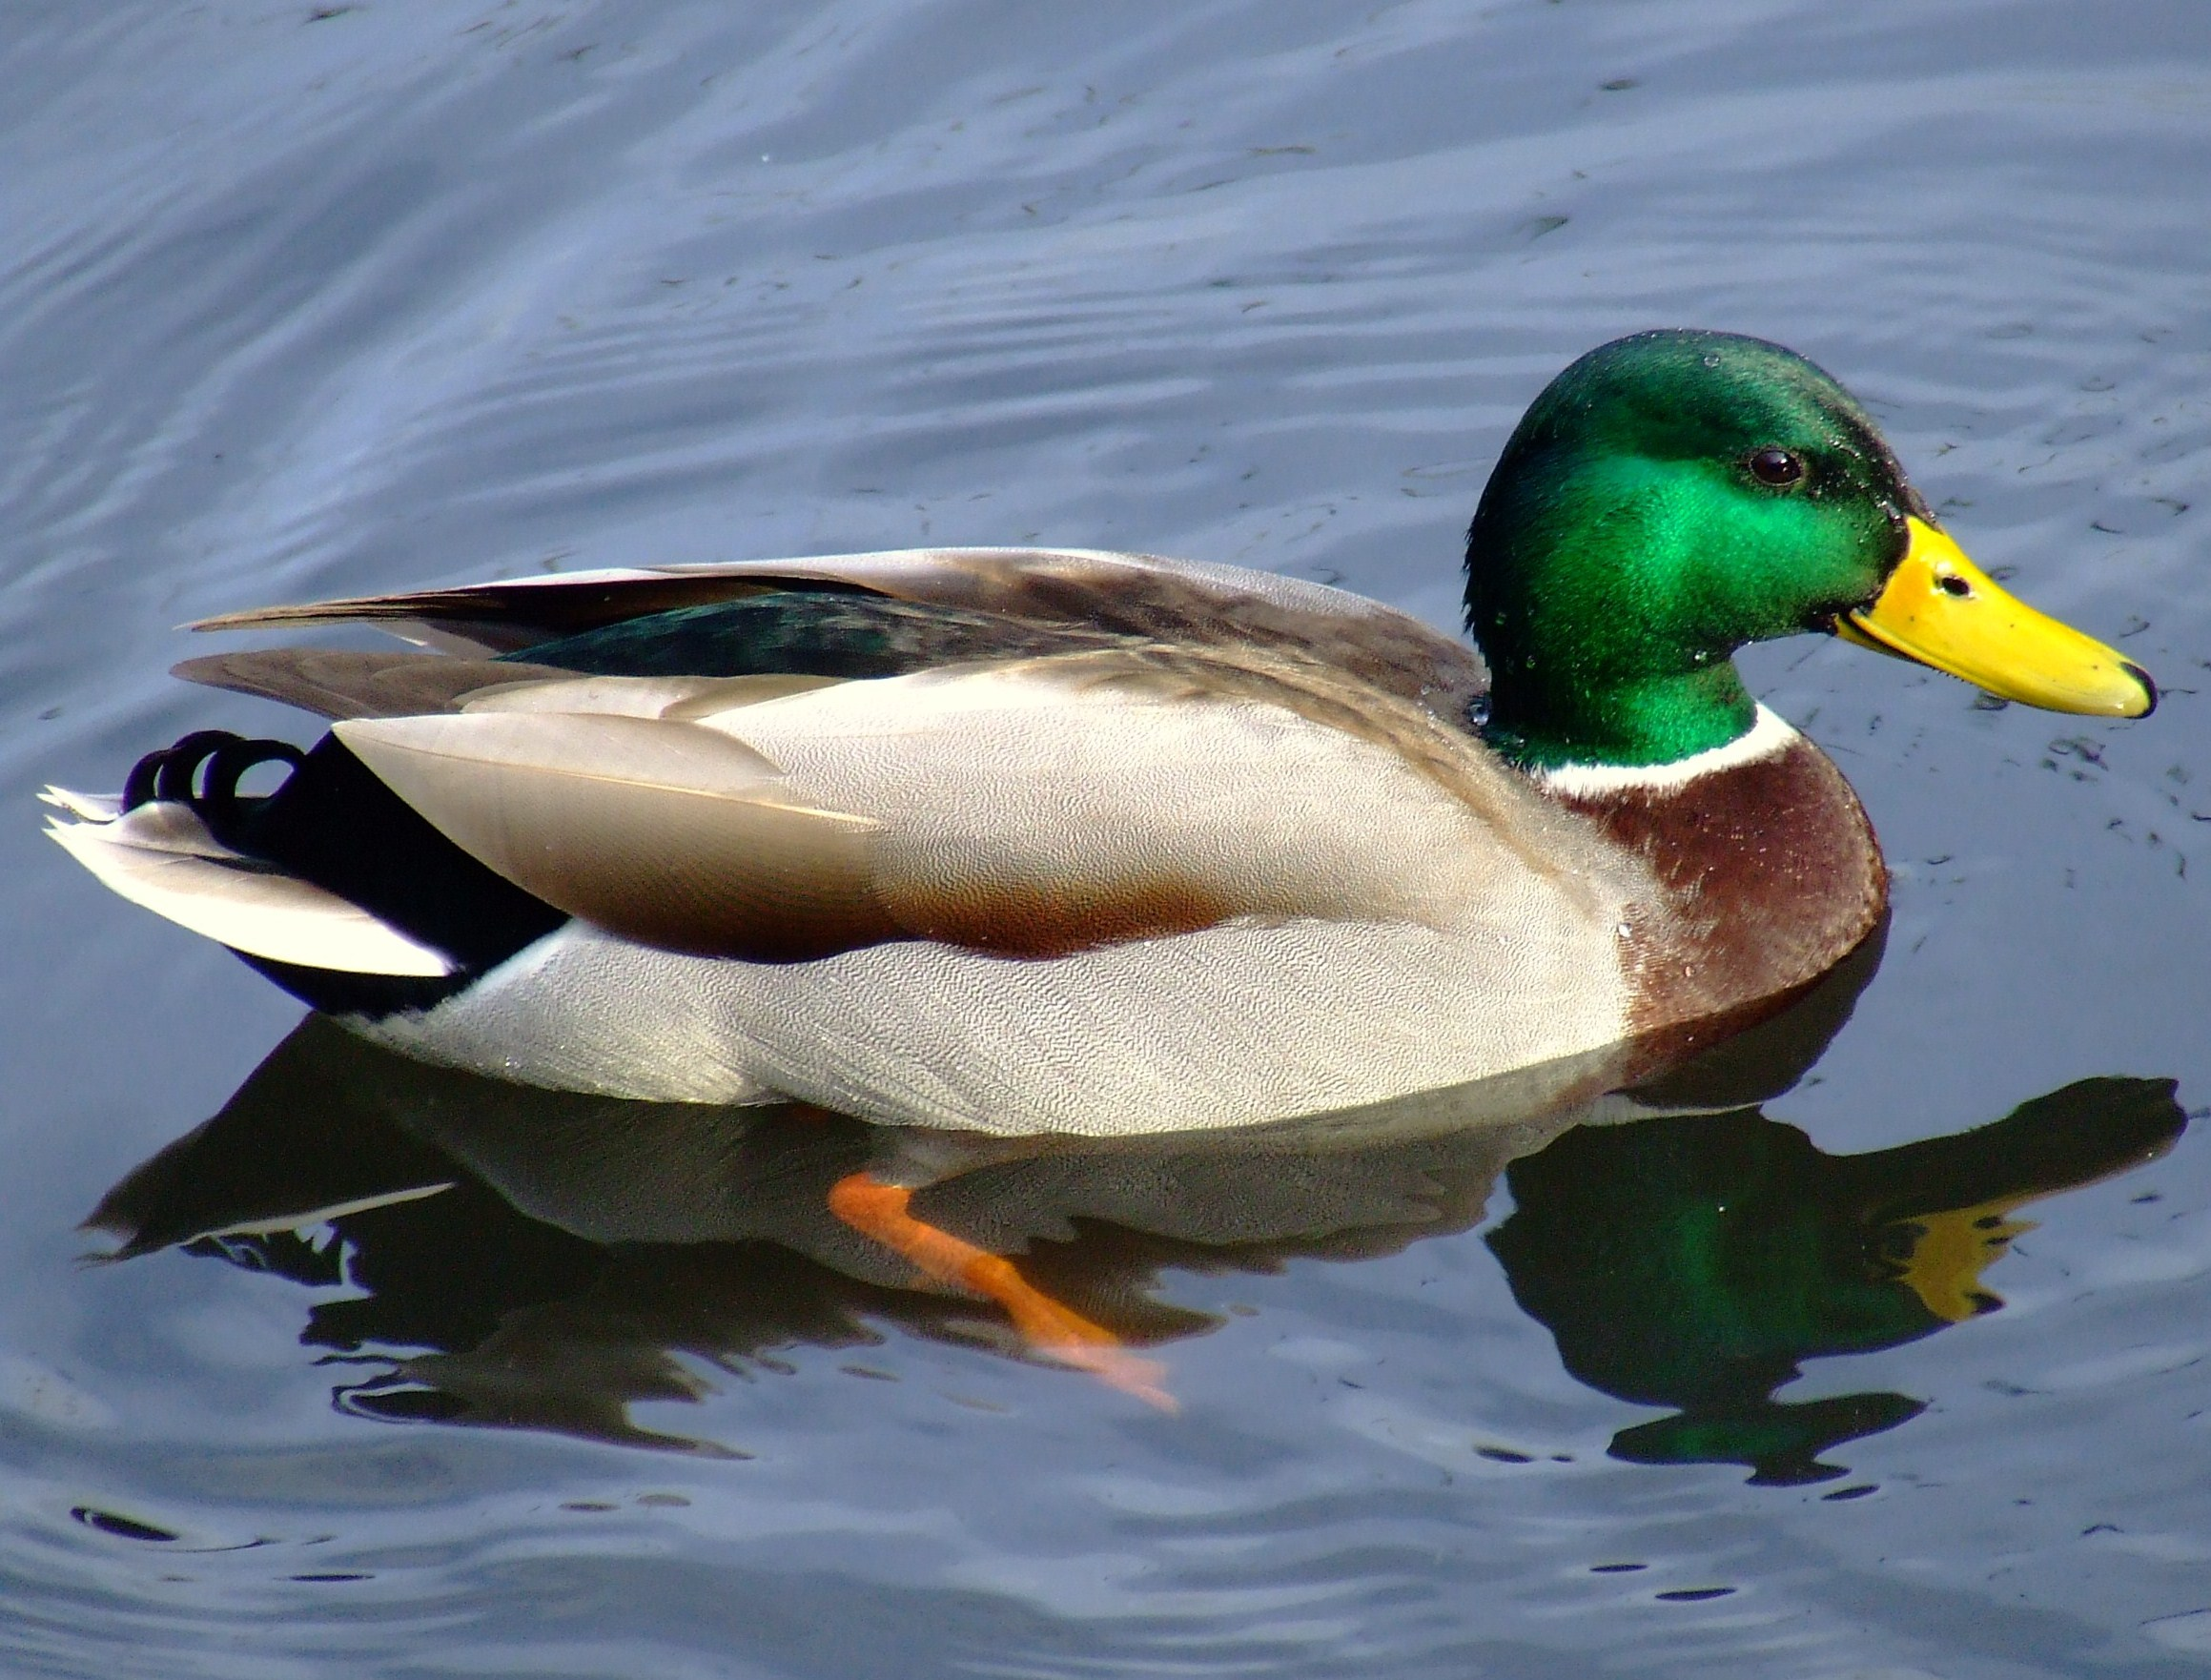
\includegraphics[width=.2\textwidth]{figs/duck1.jpg}&
         ...
         \\
        {\bf y (target)} & Cat & Dog & Duck & ...\\
    \end{tabular}
\end{table}

\end{frame}

\begin{frame}{How to proceed?}

\begin{enumerate}[<+->]
    \item Encode the targets using one hot encoding
    \begin{table}[]
    \centering
    \begin{tabular}{ccccc}
    
        {\bf y (target)} & Cat & Dog & Cat & ...\\
         {\bf y (encoded)} & $(1,0,0)$ & $(0,1,0)$ & $(0,0,1)$ & ...\\
        
    \end{tabular}
\end{table}
    \item Design a model with \alert{\bf $N$ outputs } ($N$ being the number of modalities) and use the \alert{\bf soft-max} as output activation function
    $$
       p_j=f_j(\mathbf{h}) = \frac{e^{h_j}}{\sum_k e^{h_k}}
    $$
    Rule: the class is attributed to the argument of the maximum of ${\bf p}$. Ex ${\bf p} = (0.1, 0,7, 0,2)$ is classified as ''dog''.
    \alert{\bf $p_j$ is interpreted as the probability of the image x to belong to the class $j$}
    \item Loss function to minimize is negative cross entropy
 $$L = -\sum_i \sum_j y_{i,j}.\log{p_{i,j}}$$
\end{enumerate}    
\end{frame}

\section{Optimization using gradient descent}
\begin{frame}{What is gradient descent}
\begin{block}{Objective}
Minimize the function $L(\boldsymbol{\theta})$ where $\boldsymbol{\theta}$ is a vector of parameters (e.g. weights of a neural net).
\end{block}
Example with $\boldsymbol{\theta} = (w, b)$
\begin{columns}

\column{.5\textwidth}
\begin{figure}
    \centering
    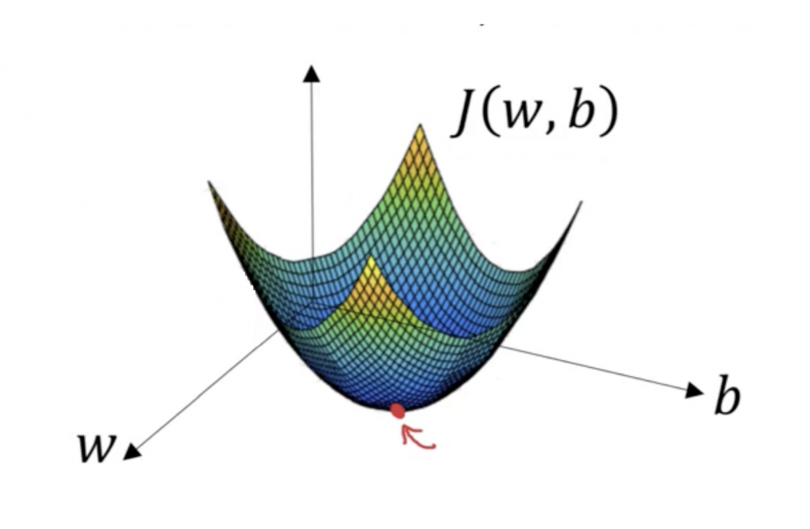
\includegraphics[width=.9\textwidth]{figs/gradient-descent-convex-function.png}
\end{figure}

\column{.5\textwidth}
\begin{figure}
    \centering
    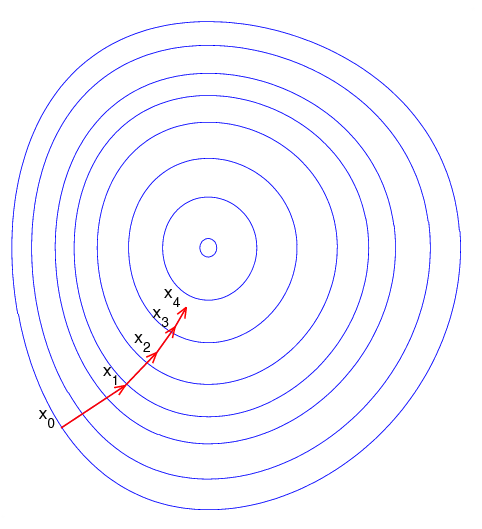
\includegraphics[width=.8\textwidth]{figs/gradient-descent-range.png}
\end{figure}
\end{columns}

\end{frame}
 \begin{frame}{Iterative algorithm}
  \begin{enumerate}[<+->]
      \item We start with a "first guess" of the parameter $\boldsymbol{\theta}_0$
      \item we iterate over several values of the parameters following the update rule:
      $$
      \boldsymbol{\theta}_{k+1} = \boldsymbol{\theta}_{k} - \gamma \nabla L(\boldsymbol{\theta}_{k}),
      $$
      $\gamma$ is called the \alert{\bf learning rate}.
  \end{enumerate}   
  \pause
  \begin{figure}
    \centering
    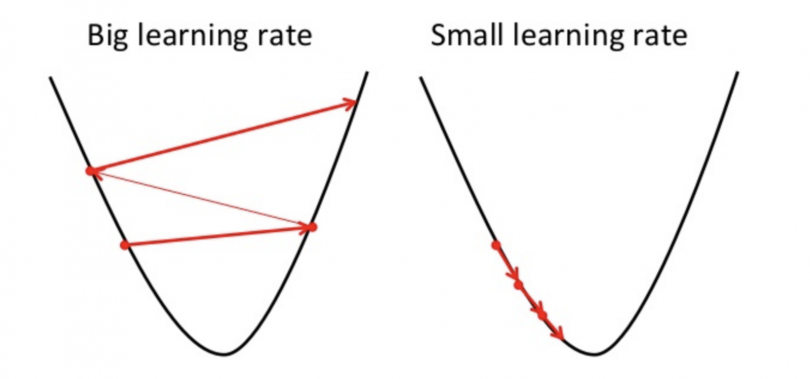
\includegraphics[width=.8\textwidth]{figs/gradient-descent-learning-rate.png}
\end{figure}
 \end{frame}

\begin{frame}{Few comments}
\begin{itemize}[<+->]
\item The learning $\gamma$ is an important \alert{\bf hyperparameter} that needs to be tuned using, e.g random search
\item The key part of the formula is the computation of the gradient $\nabla L(\boldsymbol{\theta}_{k})$
\end{itemize}
\end{frame}

\section{Gradient backpropagation}
\begin{frame}{Training a neural-net: gradient backpropagation}

\begin{columns}

\column{.5\textwidth}
\begin{figure}
    \centering
 \begin{tikzpicture}[%
    node distance = 2.5em,
    basic/.style={draw,fill=blue!20,text width=1em,text badly centered},
    input/.style={basic,circle,fill=green!20},
    output/.style={basic,circle,fill=red!20},
    weights/.style={basic,rectangle},
functions/.style={basic,circle,fill=blue!10}
]
        \node[] (center) {};
        \node[right = of center, anchor = west,output] (right) {$\hat{y}$};
        \node[above of=center,functions] (h1) {$h_1$};
        \node[below of=center,functions] (h2) {$h_2$};
        \path[draw,->] (h1) -- node[above,midway]{$w^{1}_1$}(right);
        
        \path[draw,->] (h2) --  node[below,midway]{$w^{1}_2$}(right);
        
        \node[left = of h1, input] (x1) {$x_1$};
        \node[left = of h2, input] (x2) {$x_2$};
        
        \path [draw,->] (x1) -- node[above,midway]{$w^0_{11}$} (h1);
        \path [draw,->] (x1) -- node[pos=0.25,above]{$w^0_{12}$} (h2);
        \path [draw,->] (x2) -- node[pos=0.05,above]{$w^0_{21}$} (h1);
        \path [draw,->] (x2) -- node[below,midway]{$w^0_{22}$} (h2);
\end{tikzpicture}
\end{figure}
\begin{block}{Objective}
Determination of the best set of weights $\mathbf{w}$ to minimize the Loss function $L(\mathbf{w}) = ||\hat{y}(\mathbf{w})-y||^2$.\
\alert{Calculation of $\partial L/\partial w$}
\end{block}
\column{.6\textwidth}
\begin{enumerate}[<+->]
    \item Given a couple $(x,y)$
    \item \alert{Forward computation:}\\
    $h_j  =  f_0(\sum_{i=1}^2 w^0_{ij}.x_i)$\\
$\hat{y}  =  f_1(\sum_{j=1}^2 w^1_j. h_j)$
\item \alert{Compute the gradient of the loss:~}
$\boxed{\color{red}\partial L/\partial \hat{y}}$

    \item \alert{Gradient Backpropagation:}
    \begin{itemize}
   \item Layer 1\\
   $\alert{\partial L/\partial w_j^1} = 
   \boxed{\color{red}\partial L/\partial \hat{y}}.
   \partial f_1 / \partial w^1_j$\\
   
   $ \boxed{\color{blue}\partial L/\partial h_j} = 
    \boxed{\color{red}\partial L/\partial \hat{y}}. 
   \partial f_1 / \partial h_j$
   
   \item Layer 0\\
   $\alert{\partial L/\partial w^0_{ij}}=
  \boxed{\color{blue}\partial L/\partial h_j}
   .\partial f_1 / \partial w^0_{ij}  $
    
    \end{itemize}
\end{enumerate}

\end{columns}

\end{frame}

\section{Optimizing a machine learning (gradient method)}

\begin{frame}{Optimizing the loss}
    Several loss function (depending on the problem) can be defined.
    
    For example, Mean Square Error:
    
    \begin{alertblock}{Method}
    Find a minimum of L by adjustig the parameters (weights) $\mathbf{w}$ given the gradient of the loss with respect to the weights $\nabla_\mathbf{w}L$.
    \end{alertblock}
\end{frame}



\begin{frame}{Batch Vs Stochastic training}
Dataset: $(X,Y)$ with N samples denoted $(\mathbf{x_i},y_i)$

\begin{columns}[t]
\column{.56\textwidth}
\begin{footnotesize}
\begin{block}{Batch gradient:}\end{block}
    \begin{algorithmic}
    \Require{Learning rate(s): $\nu_k$}
    \Require{Initial weights: $\mathbf{w}$}
    \State $k \leftarrow 1$
    \While {stopping criterion not met}
   % \Require{NNNN}
    %\State Sample $m$ examples ($\mathbf{x}_i,y_i)$ from ($X,y$)
    \State Compute gradient: $\mathbf{g} \leftarrow \frac{1}{N}\sum_i^N\nabla_\mathbf{w}L(f(\mathbf{x}_i,y_i))$
    \State Update weights: $\mathbf{w} \leftarrow \mathbf{w} - \nu_k\mathbf{g}$
    \State $k \leftarrow k + 1$
    \EndWhile 
    \end{algorithmic}
    \end{footnotesize}
    \alert{1 Update / N forwards}
    \pause
    \column{.56\textwidth}
\begin{footnotesize}
\begin{block}{Stochastic gradient:}\end{block}
    \begin{algorithmic}
    \Require{Learning rate(s): $\nu_k$}
    \Require{Initial weights: $\mathbf{w}$}
    \State $k \leftarrow 1$
    \While {stopping criterion not met}
   % \Require{NNNN}
    %\State Sample $m$ examples ($\mathbf{x}_i,y_i)$ from ($X,y$)
    \State Sample an example ($\mathbf{x},y)$ from ($X,Y$)
    \State Compute gradient: $\mathbf{g} \leftarrow \nabla_\mathbf{w}L(f(\mathbf{x},y))$
    \State Update weights: $\mathbf{w} \leftarrow \mathbf{w} - \nu_k\mathbf{g}$
    \State $k \leftarrow k + 1$
    \EndWhile 
    \end{algorithmic}
    \end{footnotesize}
    \alert{1 Update / 1 forward}
    
    
    \end{columns}
\end{frame}

\begin{frame}{Mini-Batch training}
Dataset: $(X,y)$ with N samples
\begin{footnotesize}
\begin{block}{Mini-Batch gradient:}\end{block}

    \begin{algorithmic}
    \Require{Learning rate(s): $\nu_k$}
    \Require{Initial weights: $\mathbf{w}$}
    \State $k \leftarrow 1$
    \While {stopping criterion not met}
   % \Require{NNNN}
    \State Sample $m$ examples ($\mathbf{x}_i,y_i)$ from ($X,y$)
    \State Compute gradient: $\mathbf{g} \leftarrow \frac{1}{m}\sum_i^m\nabla_\mathbf{w}L(f(\mathbf{x}_i,y_i)$
    \State Update weights: $\mathbf{w} \leftarrow \mathbf{w} - \nu_k\mathbf{g}$
    \State $k \leftarrow k + 1$
    \EndWhile 
    
    \end{algorithmic}
    \end{footnotesize}
    \pause
        \alert{1 Update / $m$ forward}\\
        $m=1$: Pure stochastic gradient.\\
        $m=N$: Batch gradient

\end{frame}




\end{document}